%
% qclsip: The Quantum Cascade Laser Stock Image Project.
%
% Copyright (c) 2019, Computational Photonics Group, Technical University of
% Munich.
%
% Overview of the mbsolve software.
% Created by Michael Riesch <michael.riesch@tum.de> (2019)
%
% This program is free software; you can redistribute it and/or modify
% it under the terms of the GNU General Public License as published by
% the Free Software Foundation; either version 3 of the License, or
% (at your option) any later version.
%
% This program is distributed in the hope that it will be useful,
% but WITHOUT ANY WARRANTY; without even the implied warranty of
% MERCHANTABILITY or FITNESS FOR A PARTICULAR PURPOSE.  See the
% GNU General Public License for more details.
%
% You should have received a copy of the GNU General Public License
% along with this program; if not, write to the Free Software Foundation,
% Inc., 51 Franklin Street, Fifth Floor, Boston, MA 02110-1301  USA
\documentclass[tikz]{standalone}

\usepackage[utf8]{inputenc}
\usepackage[T1]{fontenc}
\usepackage{tikz}

% set colors
\usepackage{xcolor}
\definecolor{sipblue}{RGB}{0,101,189} % Pantone 300
\definecolor{sipdarkblue}{RGB}{0,82,147} % Pantone 301
\definecolor{siplightblue}{RGB}{152,198,234} % Pantone 283
\definecolor{sipmedblue}{RGB}{100,160,200} % Pantone 542
\definecolor{sipivory}{RGB}{218,215,203} % Pantone 7527
\definecolor{sipgreen}{RGB}{162,173,0} % Pantone 383
\definecolor{siporange}{RGB}{227,114,34} % Pantone 158
\definecolor{sipgray}{gray}{0.6} % Gray 60%

% set font
\usepackage{helvet}
\renewcommand{\familydefault}{\sfdefault}

\begin{document}
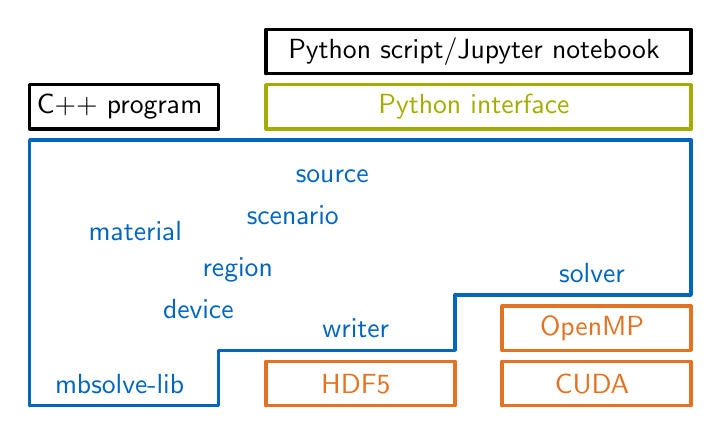
\begin{tikzpicture}
  \tikzstyle{myline}=[very thick, line cap=round,line join=round];
  \tikzstyle{mytext}=[draw=none, text=black, align=center];
  \tikzstyle{myconn}=[myline, ->, >=stealth];
  %
  % mbsolve lib
  \draw[myline, sipblue] (0, 0) -- ++(2.4, 0) -- ++(0, 20pt) -- ++(3, 0)
  -- ++(0, 20pt) -- ++(3, 0) -- ++(0, 56pt) -- ++(-8.4, 0) -- ++(0, -96pt);
  \node[mytext, sipblue] at (1.2, 8pt) { mbsolve-lib };
  \node[mytext, sipblue] at (4.2, 28pt) { writer };
  \node[mytext, sipblue] at (7.2, 48pt) { solver };
  %
  \node[mytext, sipblue] at (2.2, 35pt) { device };
  \node[mytext, sipblue] at (2.7, 49pt) { region };
  \node[mytext, sipblue] at (1.4, 63pt) { material };
  %
  \node[mytext, sipblue] at (3.4, 69pt) { scenario };
  \node[mytext, sipblue] at (3.9, 83pt) { source };
  %
  % plugins
  \draw[myline, siporange] (3, 0) -- ++(2.4, 0) -- ++(0, 16pt) --
  ++(-2.4, 0) -- ++(0, -16pt);
  \node[mytext, siporange] at (4.2, 8pt) { HDF5 };
  %
  \draw[myline, siporange] (6, 0) -- ++(2.4, 0) -- ++(0, 16pt) --
  ++(-2.4, 0) -- ++(0, -16pt);
  \node[mytext, siporange] at (7.2, 8pt) { CUDA };
  %
  \draw[myline, siporange] (6, 20pt) -- ++(2.4, 0) -- ++(0, 16pt) --
  ++(-2.4, 0) -- ++(0, -16pt);
  \node[mytext, siporange] at (7.2, 28pt) { OpenMP };
  %
  % python interface
  \draw[myline, sipgreen] (3, 100pt) -- ++(5.4, 0) -- ++(0, 16pt) --
  ++(-5.4, 0) -- ++(0, -16pt);
  \node[mytext, sipgreen] at (5.7, 108pt) { Python interface };
  %
  % application layer
  \draw[myline, black] (0, 100pt) -- ++(2.4, 0) -- ++(0, 16pt) --
  ++(-2.4, 0) -- ++(0, -16pt);
  \node[mytext, black] at (1.2, 108pt) { C++ program };
  %
  \draw[myline, black] (3, 120pt) -- ++(5.4, 0) -- ++(0, 16pt) --
  ++(-5.4, 0) -- ++(0, -16pt);
  \node[mytext, black] at (5.7, 128pt) { Python script/Jupyter notebook };
\end{tikzpicture}
\end{document}
